\documentclass[UTF8]{article} 
\usepackage{graphicx}
\usepackage{subfigure}
\usepackage{amsmath}
\usepackage{makecell}
\usepackage[utf8]{inputenc}
\usepackage[space]{ctex} %中文包
\usepackage{listings} %放代码
\usepackage{xcolor} %代码着色宏包
\usepackage{CJK} %显示中文宏包
\usepackage{float}


\definecolor{mygreen}{rgb}{0,0.6,0}
\definecolor{mygray}{rgb}{0.5,0.5,0.5}
\definecolor{mymauve}{rgb}{0.58,0,0.82}
\lstset{
	backgroundcolor=\color{white}, 
	%\tiny < \scriptsize < \footnotesize < \small < \normalsize
	basicstyle = \tiny,
	breakatwhitespace = false,        
	breaklines = true,                 
	captionpos = b,                    
	commentstyle = \color{black}\bfseries,
	extendedchars = false,             
	frame =shadowbox, 
	framerule=0.5pt,
	keepspaces=true,
	keywordstyle=\color{black}\bfseries, % keyword style
	language = C++,                     % the language of code
	otherkeywords={string}, 
	numbers=left, 
	numbersep=5pt,
	numberstyle=\tiny\color{mymauve},
	rulecolor=\color{black},         
	showspaces=false,  
	showstringspaces=false, 
	showtabs=false,    
	stepnumber=1,         
	stringstyle=\color{mymauve},        % string literal style
	tabsize=4,          
	title=\lstname                      
}
\newcommand{\jumpline} {\hspace*{\fill} \par}
\newcommand{\keypoint}[1]{$\bullet$\quad#1\par}
\newcommand{\keytitle}[2]{$\bullet$#1\quad#2\par}


\title{中国科学技术大学计算机学院\\《计算机系统概论》实验报告}
\author{}
\date{}



\begin{document}
\maketitle
\begin{figure}[H]
	\centering
	
\includegraphics[width=2.5in]{xiaohui.jpg}\vspace{0.5cm}\\
	\large{
		实验题目:HUMANOID COMPILER\\
		学生姓名:王章瀚\\
		学生学号:PB18111697\\
		完成日期:\today\\
	}\vspace{2cm}
	
	\large{计算机实验教学中心制\\2019年09月\\}
	\thispagestyle{empty}
	\clearpage  % 清除当页页码
\end{figure}



\section{实验要求}
\subsection{总述}
手动完成给定C语言代码到LC-3汇编码的编译,并将它编译为LC-3的object文件。
\subsection{C代码源码}
\begin{figure}[H]
	\centering
	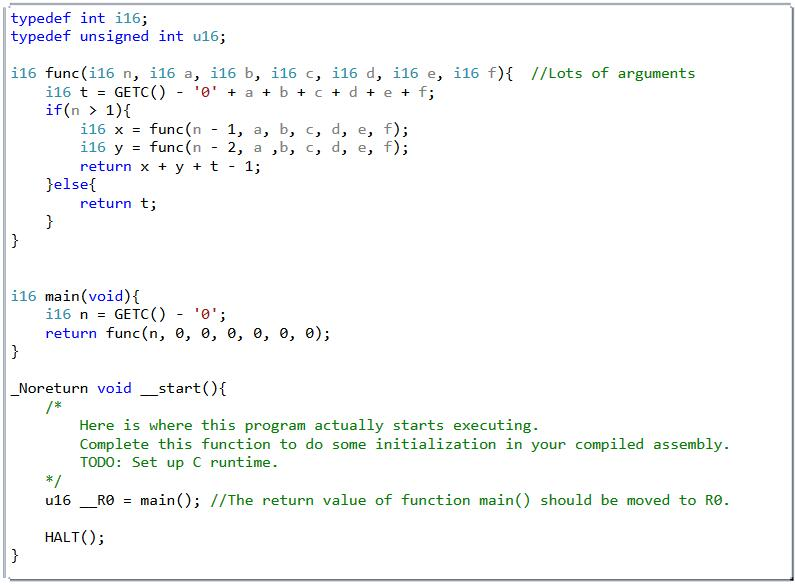
\includegraphics[scale=0.5]{C_code.jpg}
	\label{C_code}
\end{figure}\par
\subsection{细节要求}
\keypoint{应按照C标准,并完全遵照原代码进行翻译。不要对代码做任何优化,甚至改变其控制流结构。}
\keypoint{不得使用任何第三方C编译器。}
\keypoint{\_\_start()不是一个函数。它标志着程序由此开始,并调用main函数。由于最开始寄存器和内存空间都是随机的,你需要自己设计并完成初始化过程。这个过程应该要是通用的,这意味着它和main函数或其他函数的内容无关。}
\keypoint{GETC()和HALT()是TRAP。因此请做出一个TRAP应该遵循的标准,使得你的程序不会被打乱。请注意你程序中所有的调用也应该遵循这个标准。}
\keypoint{如果有程序想调用你的程序中的func(),它应该遵循某些规则,请设计这些规则。请注意你的程序里的调用也应该遵循这个规则。}
\keypoint{你的程序会被随机地载入到x3000-xC000。因此object文件的.ORIG和前两个字节将被忽略。}
\keypoint{实验报告应该包含:1.初始化过程;2.调用约定;3.其他你设计的标准;4.错误处理。}



\section{设计思路}
\subsection{总体思路}
观察可知,C源码中,除了main函数,只有一个func函数,而该函数会被递归调用。因此需要考虑函数栈。其他的由于是翻译,并没有太多需要注意的,只需要照着翻译即可。而为了方便,不再按照书上使用FramePointer的方法,而是直接通过函数栈指针(这里用R6)的偏移来访问每个栈元素的各个子元素。\par
\subsection{初始化过程}
此处似乎并不需要做任何初始化。但为了好看,将所有寄存器初始化为0,并读取栈指针位置到R6。\par
\begin{lstlisting}[language=C++]
AND	R0, R0, #0
AND	R1, R1, #0
AND	R2, R2, #0
AND	R3, R3, #0
AND	R4, R4, #0
AND	R5, R5, #0
AND	R6, R6, #0
AND	R7, R7, #0
LD	R6, func_stack	;读取栈初始地址
\end{lstlisting}
\subsection{调用约定}
\subsubsection{TRAP标准}
\keypoint{程序中所有有调用了TRAP的地方,都应该\textbf{提前保存R7},并在需要用到之前将R7重新载回。(例如程序中使用的GETC,应保存R7,否则将无法正常返回。)}
\subsubsection{func函数标准}
\keypoint{要想使用func函数,必须有一个寄存器或一个内存空间来\textbf{保存func函数栈指针}。本例中始终用R6保存。}
\keypoint{本函数\textbf{不对寄存器进行任何保存处理},如有需要,请在调用前自行保存}
\keypoint{函数栈空间说明:\par
	栈空间起始位置是由汇编代码:\textbf{func\_stack\quad.FILL\quad xD000}决定,\underline{起始位置即该处值}。如此时,则从\textbf{xD000}开始。\par
	栈空间大小由汇编代码:\textbf{stack\_size\quad.FILL\quad x1C2C}决定。\underline{大小为该处值-xC}。如此时,大小为x1C2C-xC=\textbf{x1C20}。\par
	栈空间中,每个元素为一块,\textbf{每块12个内存空间},其含义如下表:\par
	\begin{figure}[H]
		\centering
		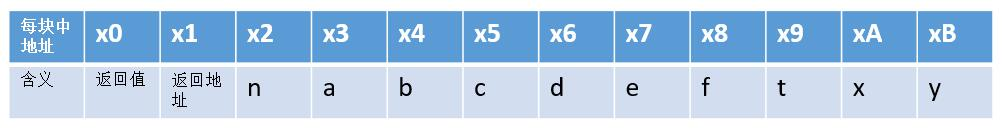
\includegraphics[scale=0.5]{stack.jpg}
		\label{stack}
	\end{figure}\par
%	\begin{table}[H]
%		\small
%		\begin{tabular}{|c|c|c|c|c|c|c|c|c|c|c|c|c|}
%			\hline 
%			每块中地址 & x0 & x1 & x2 & x3 & x4 & x5 & x6 & x7 & x8 & x9 & xA & xB \\ 
%			\hline 
%			含义 & 返回值 & 返回地址 & n & a & b & c & d & e & f & t & x & y \\ 
%			\hline 
%		\end{tabular}
%	\end{table}
}
\jumpline
\keypoint{在调用func函数之前,应使R6向后偏移\textbf{12}个内存地址空间,并将\textbf{所有参数通过R6对应入栈}。例如:将参数a的值存入偏移后R6+3处。}
\keypoint{函数的返回:函数返回时,R6\textbf{不会}回退到调用处的栈位置,这是为了读取返回值方便,\textbf{如调用func,请手动进行回退};如需要读取返回值,可以通过\textbf{R6+x0}获取。}
\subsection{错误处理}
设计中,会出现的错误在于栈空间溢出,即超出了前述stack\_size-xC的大小。对此进行的处理是,每次调用时检测 \textbf{R6-栈起始位置} 是否达到了栈空间大小,如果达到,则输出"Stack OverFlow!"。\par



\section{关键代码讲解}
因为是翻译,没有什么比较特别的地方需要特别说明,因此以下只将代码贴出,并在后面按行说明。\par
\subsection{func函数}
先放出代码:\par
\begin{lstlisting}[language=C++]
func			STR	R7, R6, #1	; 存好R7所保存的返回地址
				GETC			; 计算t开始
				LD	R1, c_n30	
				ADD	R0, R0, R1	; t-='0'
				LDR	R1, R6, #3	; 从内存读取a
				ADD	R0, R0, R1	; 加上a
				LDR	R1, R6, #4	; 从内存读取b
				ADD	R0, R0, R1	; 加上b
				LDR	R1, R6, #5	; 从内存读取c
				ADD	R0, R0, R1	; 加上c
				LDR	R1, R6, #6	; 从内存读取d
				ADD	R0, R0, R1	; 加上d
				LDR	R1, R6, #7	; 从内存读取e
				ADD	R0, R0, R1	; 加上e
				LDR	R1, R6, #8	; 从内存读取f	
				ADD	R0, R0, R1	; 加上f, 计算t结束
				STR	R0, R6, #9	; 存放t
				
				LDR	R1, R6, #2	; 读取n
				ADD	R2, R1, #-1	; 计算n-1
				BRnz	ELSE	; 若n-1<=0,跳转到ELSE
				
				ADD	R6, R6, #12	; 将R6指向下一个栈空间,为下一次递归调用做准备
				LD	R3, stack_size	; 读取栈空间总大小
				LD	R4, func_stack	; 读取栈空间起始位置
				ADD	R3, R3, R4	; 计算栈空间末尾位置
				NOT	R3, R3
				ADD	R3, R3, #1	; 计算栈空间末位置的相反数
				ADD	R3, R3, R6	; R6-栈空间末位置
				BRz	stackoverflow	; 栈溢出
				LDR	R1, R6, #-10	; 从内存读取n
				ADD	R2, R1, #-1	; 求n-1
				STR	R2, R6, #2	; 存到R6+#2上
				LDR	R1, R6, #-9	; 从内存读取a
				STR	R1, R6, #3	; 存到R6+#3上
				LDR	R1, R6, #-8	; 从内存读取b
				STR	R1, R6, #4	; 存到R6+#4上
				LDR	R1, R6, #-7	; 从内存读取c
				STR	R1, R6, #5	; 存到R6+#5上
				LDR	R1, R6, #-6	; 从内存读取d
				STR	R1, R6, #6	; 存到R6+#6上
				LDR	R1, R6, #-5	; 从内存读取e
				STR	R1, R6, #7	; 存到R6+#7上
				LDR	R1, R6, #-4	; 从内存读取f
				STR	R1, R6, #8	; 存到R6+#8上
				JSR	func		; 递归调用以求x
				LDR	R0, R6, #0	; 读取递归调用求x得到的返回值
				STR	R0, R6, #-2	; 存在当前栈的x空间位置上
				LDR	R1, R6, #-10	; 从内存读取n
				ADD	R2, R1, #-2	; 求n-2
				STR	R2, R6, #2	; 存到 R6+#2 上
				; 其余R1到R6上一次均已经存好,且未改变
				JSR	func		; 递归调用以求y
				LDR	R0, R6, #0	; 读取递归调用求y得到的返回值
				STR	R0, R6, #-1	; 存在当前栈的y空间位置上
				
				ADD	R6, R6, #-12	; 栈指针指回当前调用函数对应栈
				
				LDR	R0, R6, #9	; 读取t到R0
				LDR	R1, R6, #10	; 读取x到R1
				ADD	R0, R0, R1	; 求t+x
				LDR	R1, R6, #11	; 读取y到R1
				ADD	R0, R0, R1	; 求t+x+y
				ADD	R0, R0, #-1	; 求t+x+y-1
				STR	R0, R6, #0	; 返回值存在R6+#0
				
				LDR	R7, R6, #1	; 读取R7所保存的返回地址
				RET			; 以上完成了n>1的情况
				;以下是n<=1的情况
ELSE			LDR	R0, R6, #9	; 返回t,把t的值读入R0
				STR	R0, R6, #0	; 返回值存在R6+#0
				LDR	R7, R6, #1	; 读取R7所保存的返回地址
				RET			; n<=1,直接返回
stackoverflow	LEA	R0, sof_message
				PUTS
				HALT
				
sof_message		.STRINGZ "Stack OverFlow!"	
c_n30			.FILL	x-30		; '0'的ASCII的相反数 
stack_size		.FILL	x1C2C		; 栈的大小+#12, x1C2C+#12=#7212
func_stack		.FILL	xD000		; 为func函数的栈保留空间
\end{lstlisting}\par
以下按行说明代码:\par
\keytitle{Line1-2}{存R7, GETC读数}
\keytitle{Line3-17}{计算t,并存入函数栈空间}
\keytitle{Line19-21}{分支语句,判断n}
\keytitle{Line23-30}{n>1,准备递归调用,判断是否栈溢出}
\keytitle{Line31-45}{传参过程}
\keytitle{Line46-48}{调用函数,保存返回值到x}
\keytitle{Line49-51}{传参过程}
\keytitle{Line53-55}{调用函数,保存返回值到y}
\keytitle{Line57}{func栈指针回退}
\keytitle{Line59-65}{计算t+x+y-1,并存在返回值位置上}
\keytitle{Line67-68}{n>1时的返回}
\keytitle{Line70-73}{n<=1时的返回}
\keytitle{Line74-76}{栈溢出处理}
以上就是对func函数的编写进行的阐述,代码注释也比较清晰。\par
\subsection{main函数}
先放出代码:\par
\begin{lstlisting}[language=C++]
main		ST	R7, main_R7	;存好R7所保存的返回地址
			GETC
			LD	R1, c_n30
			ADD	R1, R0, R1	;计算初始n
			LD	R6, func_stack	;读取栈初始地址
			STR	R1, R6, #2	;把n存到R6+#1上
			AND	R1, R1, #0	;初始化R1为0
			STR	R1, R6, #3	;a处存为0
			STR	R1, R6, #4	;b处存为0
			STR	R1, R6, #5	;c处存为0
			STR	R1, R6, #6	;d处存为0
			STR	R1, R6, #7	;e处存为0
			STR	R1, R6, #8	;f处存为0
			JSR	func		;调用func
			LDR	R0, R6, #0	;读取返回值
			ADD	R6, R6, #-12	;R6回退
			ST	R0, main_ret	;返回值写到main函数返回值处
			LD	R7, main_R7
			RET
main_ret	.BLKW	1
main_R7		.BLKW	1
\end{lstlisting}\par
这段代码对func函数进行了一次调用,中间一大部分都是在进行传参操作。\par
其他则是一些初始化,返回等操作,已注释清楚。\par



\section{调试分析}
\subsection{正常数据测试}
设当main函数中,输入为字符c时,后面还需要输入n(c)个字符。\par
通过计算,可以知道
$$
\left\{
\begin{array}{l}
n(0)=1\\
n(1)=1\\
n(c+2)=n(c+1)+n(c)+1\\
\end{array}
\right. 
$$\par
这是后续数据选取的依据。\par
以下随机选取了两组测试数据及取了一组00的测试数据:\par
\subsubsection{测试数据1}
测试时输入:54896518461sagg6\par
可以看到最终R0得到了:277.\par
这与实际结果相同:
\begin{figure}[H]
	\begin{minipage}[H]{0.48\linewidth}
		\centering
		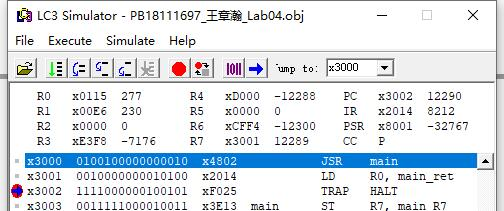
\includegraphics[scale=0.45]{test1.jpg}
		\caption{测试结果}
		\label{test1}
	\end{minipage}
	\qquad
	\begin{minipage}[H]{0.48\linewidth}
		\centering
		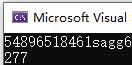
\includegraphics[scale=1]{test1_a.jpg}
		\caption{实际结果}
		\label{test1_a}
	\end{minipage}
\end{figure}
\subsubsection{测试数据2}
测试时输入:6f14ge687941aeo6u52f13v267\par
可以看到最终R0得到了:580.\par
这与实际结果相同:
\begin{figure}[H]
\begin{minipage}[H]{0.48\linewidth}
	\centering
	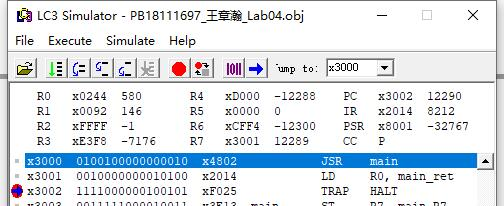
\includegraphics[scale=0.45]{test2.jpg}
	\caption{测试结果}
	\label{test2}
\end{minipage}
\qquad
\begin{minipage}[H]{0.48\linewidth}
	\centering
	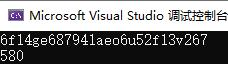
\includegraphics[scale=1]{test2_a.jpg}
	\caption{实际结果}
	\label{test2_a}
\end{minipage}
\end{figure}
\subsubsection{测试数据3}
测试时输入:00\par
可以看到最终R0得到了:0.\par
这与实际结果相同:
\begin{figure}[H]
\begin{minipage}[H]{0.48\linewidth}
	\centering
	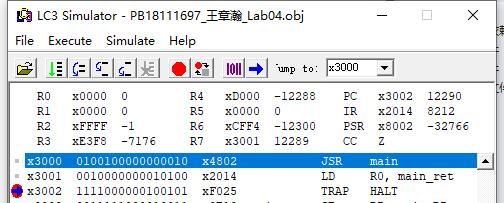
\includegraphics[scale=0.45]{test3.jpg}
	\caption{测试结果}
	\label{test3}
\end{minipage}
\qquad
\begin{minipage}[H]{0.48\linewidth}
	\centering
	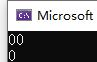
\includegraphics[scale=1]{test3_a.jpg}
	\caption{实际结果}
	\label{test3_a}
\end{minipage}
\end{figure}
\subsection{异常数据测试}
由于输入不便,测试栈溢出的时候,缩小栈空间来测试。
设置栈空间为\#36-xB=\#24,令输入为5555,则会有如下提示:\par
\begin{figure}[H]
	\centering
	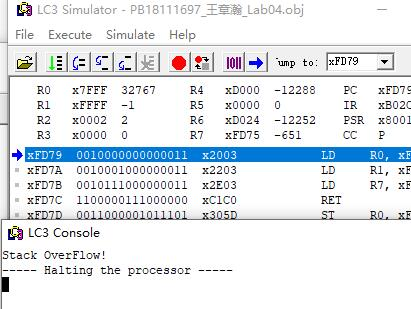
\includegraphics[scale=0.5]{sof.jpg}
	\caption{函数栈溢出}
	\label{sof}
\end{figure}\par



\section{Great Idea}
本程序中,将函数中所有的参数,变量都当作一个栈元素的整体压入栈中,这将对程序日后需要的拓展提供了很大方便。且这样的思路,是完全可以作为C to LC-3汇编码的编译器中函数的处理思路。因为它所有的变量读取与赋值,不是依赖于寄存器的使用,而主要是直接靠内存读写。\par



\section{实验总结}
本次实验中,实现了函数的递归调用操作,这其中运用的栈思想是十分重要的。通过栈的使用,可以避免参数丢失,又能满足函数调用的FILO的规律。相信它在日后的计算机的学习中,将有很大作用。



\section{附录:完整的LC-3汇编代码}
\begin{lstlisting}[language=C++]
				.ORIG	x3000
				AND	R0, R0, #0
				AND	R1, R1, #0
				AND	R2, R2, #0
				AND	R3, R3, #0
				AND	R4, R4, #0
				AND	R5, R5, #0
				AND	R6, R6, #0
				AND	R7, R7, #0
				JSR	main
				LD	R0, main_ret	;读取返回值
				HALT

main			ST	R7, main_R7	;存好R7所保存的返回地址
				GETC
				LD	R1, c_n30
				ADD	R1, R0, R1	;计算初始n
				LD	R6, func_stack	;读取栈初始地址
				STR	R1, R6, #2	;把n存到R6+#1上
				AND	R1, R1, #0	;初始化R1为0
				STR	R1, R6, #3	;a处存为0
				STR	R1, R6, #4	;b处存为0
				STR	R1, R6, #5	;c处存为0
				STR	R1, R6, #6	;d处存为0
				STR	R1, R6, #7	;e处存为0
				STR	R1, R6, #8	;f处存为0
				JSR	func		;调用func
				LDR	R0, R6, #0	;读取返回值
				ADD	R6, R6, #-12	;R6回退
				ST	R0, main_ret	;返回值写到main函数返回值处
				LD	R7, main_R7
				RET
main_ret		.BLKW	1
main_R7			.BLKW	1

func			STR	R7, R6, #1	;存好R7所保存的返回地址
				GETC			;计算t开始
				LD	R1, c_n30	
				ADD	R0, R0, R1	;t-='0'
				LDR	R1, R6, #3	;从内存读取a
				ADD	R0, R0, R1	;加上a
				LDR	R1, R6, #4	;从内存读取b
				ADD	R0, R0, R1	;加上b
				LDR	R1, R6, #5	;从内存读取c
				ADD	R0, R0, R1	;加上c
				LDR	R1, R6, #6	;从内存读取d
				ADD	R0, R0, R1	;加上d
				LDR	R1, R6, #7	;从内存读取e
				ADD	R0, R0, R1	;加上e
				LDR	R1, R6, #8	;从内存读取f	
				ADD	R0, R0, R1	;加上f, 计算t结束
				STR	R0, R6, #9	;存放t
				
				LDR	R1, R6, #2	;读取n
				ADD	R2, R1, #-1	;计算n-1
				BRnz	ELSE		;若n-1<=0,跳转到ELSE
				
				ADD	R6, R6, #12	;将R6指向下一个栈空间,为下一次递归调用做准备
				LD	R3, stack_size	;读取栈空间总大小
				LD	R4, func_stack	;读取栈空间起始位置
				ADD	R3, R3, R4	;计算栈空间末尾位置
				NOT	R3, R3
				ADD	R3, R3, #1	;计算栈空间末位置的相反数
				ADD	R3, R3, R6	;R6-栈空间末位置
				BRz	stackoverflow	;栈溢出
				LDR	R1, R6, #-10	;从内存读取n
				ADD	R2, R1, #-1	;求n-1
				STR	R2, R6, #2	;存到R6+#2上
				LDR	R1, R6, #-9	;从内存读取a
				STR	R1, R6, #3	;存到R6+#3上
				LDR	R1, R6, #-8	;从内存读取b
				STR	R1, R6, #4	;存到R6+#4上
				LDR	R1, R6, #-7	;从内存读取c
				STR	R1, R6, #5	;存到R6+#5上
				LDR	R1, R6, #-6	;从内存读取d
				STR	R1, R6, #6	;存到R6+#6上
				LDR	R1, R6, #-5	;从内存读取e
				STR	R1, R6, #7	;存到R6+#7上
				LDR	R1, R6, #-4	;从内存读取f
				STR	R1, R6, #8	;存到R6+#8上
				JSR	func		;递归调用以求x
				LDR	R0, R6, #0	;读取递归调用求x得到的返回值
				STR	R0, R6, #-2	;存在当前栈的x空间位置上
				LDR	R1, R6, #-10	;从内存读取n
				ADD	R2, R1, #-2	;求n-2
				STR	R2, R6, #2	;存到R6+#2上
				;其余R1到R6上一次均已经存好,且未改变
				JSR	func		;递归调用以求y
				LDR	R0, R6, #0	;读取递归调用求y得到的返回值
				STR	R0, R6, #-1	;存在当前栈的y空间位置上
				
				ADD	R6, R6, #-12	;栈指针指回当前调用函数对应栈
				
				LDR	R0, R6, #9	;读取t到R0
				LDR	R1, R6, #10	;读取x到R1
				ADD	R0, R0, R1	;求t+x
				LDR	R1, R6, #11	;读取y到R1
				ADD	R0, R0, R1	;求t+x+y
				ADD	R0, R0, #-1	;求t+x+y-1
				STR	R0, R6, #0	;返回值存在R6+#0
				
				LDR	R7, R6, #1	;读取R7所保存的返回地址
				RET				;以上完成了n>1的情况
								;以下是n<=1的情况
ELSE			LDR	R0, R6, #9	;返回t,把t的值读入R0
				STR	R0, R6, #0	;返回值存在R6+#0
				LDR	R7, R6, #1	;读取R7所保存的返回地址
				RET			;n<=1,直接返回
				stackoverflow	LEA	R0, sof_message
				PUTS
				HALT


sof_message		.STRINGZ "Stack OverFlow!"	
c_n30			.FILL	x-30		;'0'的ASCII的相反数
;stack_size		.FILL	#36		
stack_size		.FILL	x1C2C		;栈的大小+#12, x1C2C+#12=#7212
func_stack		.FILL	xD000		;为func函数的栈保留空间
									;func函数栈空间存储按照下述格式:
									;1. 每12个内存地址为一块
									;2. 每块顺序存放:
									;	x0	返回值
									;	x1	RET应返回到的R7
									;	x2	n
									;	x3	a
									;	x4	b
									;	x5	c
									;	x6	d
									;	x7	e
									;	x8	f
									;	x9	t
									;	xA	x
									;	xB	y
									
									.END
\end{lstlisting}\par
	
	
\end{document}
